\documentclass{bmvc2k}

%% Enter your paper number here for the review copy
% \bmvcreviewcopy{??}

\usepackage{float}
% \usepackage[brazilian]{babel}
\usepackage[utf8]{inputenc}

\title{Calibração de Camera}

% Enter the paper's authors in order
% \addauthor{Name}{email/homepage}{INSTITUTION_CODE}
\addauthor{Abdullah Zaiter\\15/0089392}{abdullah.zaiter@gmail.com}{1}
\addauthor{Ian Moura Alexandre\\15/0129661}{ianzeba@gmail.com}{1}


% Enter the institutions
% \addinstitution{Name\\Address}
\addinstitution{
  Departamento de Ci\^encia da Comptuta\c{c}\~ao\\
  Universidade de Bras\'{\i}lia\\
  Campus Darcy Ribeiro, Asa Norte\\
  Bras\'{\i}lia-DF, CEP 70910-900, Brazil,  
}

\runninghead{Zaiter, Abdullah-Alexandre, M. Ian}{Calibração de camera -- \today}

% Any macro definitions you would like to include
% These are not defined in the style file, because they don't begin
% with \bmva, so they might conflict with the user's own macros.
% The \bmvaOneDot macro adds a full stop unless there is one in the
% text already.
\def\eg{\emph{e.g}\bmvaOneDot}
\def\Eg{\emph{E.g}\bmvaOneDot}
\def\etal{\emph{et al}\bmvaOneDot}

%-------------------------------------------------------------------------
% Document starts here
\begin{document}

\maketitle

\begin{abstract}
Este documento apresenta os fundamentos teóricos, a metologia e os resultados obtidos para a implementação de um algoritmo para calibração de uma câmera usando OpenCV \cite{opencv_library} e, com os parâmetros conhecidos da câmera , o desenvolvimento de um sistema de medição utilizando-se a {\em webcam}.
\end{abstract}

%-------------------------------------------------------------------------
\section{Introdução}
\label{sec:intro}
\footnote{Abdullah: Desenvolveu o método de calibração de intrínsecos e extrínsecos, e desenvolveu parte da parte da régua visual. No relatório, foi responsável pela Conclusão e Resultados.}.
\footnote{Ian: Desenvolveu a primeira parte do projeto, com a medição da distância entre dois píxels, ajudou no desenvolvimento da régua visual. No relatório, escreveu a introdução e desenvolvimento.}
Fazendo-se uso da câmera como um sensor quantitativo, torna-se essencial a sua calibração. A calibração é uma estimação de um modelo não-configurado de câmera, com o intuito de se haver correspondência entre pontos na imagem e pontos no espaço, como dito em \cite{Horn01}. Para isso, acha-se a matriz de projeção M e os parâmetros intrínsecos e extrínsecos.\\
A matriz de projeção apresenta qual é a proporção entre a imagem obtida da imagem da câmera para os objetos no mundo real, obtendo assim o que seria referente a distância focal da câmera. Os modelos utilizados para tal projeção é o modelo {\em pinhole}, também chamado de modelo de câmera de Tsai \cite{Dias01}, em que a sua representação em coordenadas homogêneas é representada pela equação \ref{homogeneosPinhole}, sendo a matriz M uma matriz de dimensões 3x4, onde f representaria o zoom da imagem.\\

\begin{equation}\label{homogeneosPinhole}
\left( \begin{array}{l}{\tilde{x}} \\ {\tilde{y}} \\ {\tilde{z}}\end{array}\right)=\left( \begin{array}{llll}{f} & {0} & {0} & {0} \\ {0} & {f} & {0} & {0} \\ {0} & {0} & {1} & {0}\end{array}\right) \left( \begin{array}{l}{X} \\ {Y} \\ {Z} \\ {1}\end{array}\right)
\end{equation}
Para o modelo de uma câmera completa, necessita-se considerar os fatores que podem afetar esta projeção, sendo estes os fatores intrínsecos e extrínsecos. Os fatores intrínsecos são aqueles referentes à aspectos de hardware da câmera, sendo um destes o tamanho dos píxels e seu formato. Dessa forma, é necessário que a matriz M seja dividida pela quantidade de píxels da imagem e o seu referencial levado para o canto esquerdo da imagem. Os fatores extrínsecos são dependentes das posições linear e angular da câmera. Dessa forma, obtém-se a equação \ref{homogeneousCam}, formando-se com as três matrizes a matriz da câmera.\\

\begin{equation}\label{homogeneousCam}
    \left( \begin{array}{c}{\tilde{u}} \\ {\tilde{v}} \\ {\tilde{w}}\end{array}\right)=\left( \begin{array}{ccc}{\frac{1}{\rho_{u}}} & {0} & {u_{0}} \\ {0} & {\frac{1}{\rho_{v}}} & {v_{0}} \\ {0} & {0} & {1}\end{array}\right) \left( \begin{array}{cccc}{f} & {0} & {0} & {0} \\ {0} & {f} & {0} & {0} \\ {0} & {0} & {1} & {0}\end{array}\right) \left( \begin{array}{cc}{\mathbf{R}} & {t} \\ {\mathbf{0}_{1 \times 3}} & {1}\end{array}\right)^{-1} \left( \begin{array}{c}{X} \\ {Y} \\ {Z} \\ {1}\end{array}\right)
\end{equation}

Entretanto, o mais comum é que se tenha uma matriz com doze elementos, como obtido na equação \ref{camMatrix} e à partir dele é estimado seus valores. Para simplificar a matriz estimada, coloca-se o referencial do mundo no plano do ponto desejado, além de que como o fator de escala na homografia é arbitrário, como mostrado em \cite{Opencv02}, obtém-se a equação homográfica \ref{camFinal}, com 8 parâmetros.
\begin{equation}\label{camMatrix}
    \left( \begin{array}{c}{\tilde{u}} \\ {\tilde{v}} \\ {\tilde{w}}\end{array}\right)=\lambda \left( \begin{array}{cccc}{C_{11}} & {C_{12}} & {C_{13}} & {C_{14}} \\ {C_{21}} & {C_{22}} & {C_{23}} & {C_{24}} \\ {C_{31}} & {C_{32}} & {C_{33}} & {C_{34}}\end{array}\right) \left( \begin{array}{l}{X} \\ {Y} \\ {Z} \\ {1}\end{array}\right)
\end{equation}
\begin{equation}\label{camFinal}
    \left( \begin{array}{c}{\tilde{u}} \\ {\tilde{v}} \\ {\tilde{w}}\end{array}\right)=\left( \begin{array}{lll}{C_{11}} & {C_{12}} & {C_{14}} \\ {C_{21}} & {C_{22}} & {C_{24}} \\ {C_{31}} & {C_{32}} & {1}\end{array}\right) \left( \begin{array}{l}{X} \\ {Y} \\ {1}\end{array}\right)
\end{equation}

Tendo a equação \ref{homogeneousCam}, a calibração é feita por meio da correspondência de pontos entre diferentes imagens e, sabendo-se um referencial de medida do mundo, pode-se estimar uma homografia e assim mapear pontos na imagem. As aplicações para este tipo de técnica de calibração são diversas, como estimação da posição da cabeça\cite{Opencv100}, e a realização de medidas em centímetros utilizando-se a transmissão de webcam, como discutido neste documento.\\

\section{Desenvolvimento}
Para melhor controle de versão e rastreamento de mudanças, utilizou-se a ferramenta Git em um \href{https://github.com/abdullah-zaiter/Camera-Calibration}{Repositório} do autor no site GitHub.\\
Para o algoritmo realizado, escolheu-se desenvolvê-lo utilizando a linguagem Python, sendo grande parte das funções utilizadas oriundas da biblioteca de visão computacional \href{https://opencv.org/}{OpenCV}\cite{opencvrefman}. Para a montagem do código, dividiu-se em quatro requisitos:
\begin{itemize}
    \item Calcular a distância entre dois píxels da imagem 
    \item Calibração dos Parâmetros Intrínsecos
    \item Calibração dos Parâmetros Extrínsecos
    \item Desenvolvimento da Régua Visual
\end{itemize}

\subsection{Distância entre dois pontos na imagem}
\label{subsubsec: Dist}
Na execução desta parte do algoritmo, solicita-se do usuário o índice de sua câmera e em seguida começa-se a transmissão de sua imagem. Para capturar o sinal do mouse do usuário, utiliza-se a função do OpenCV \href{https://docs.opencv.org/2.4/modules/highgui/doc/user_interface.html?highlight=setmousecallback#setmousecallback}{cv2.SetMouseCallback}, sendo chamado a função \small{get\_mouse\_clicks}. Nesta função, espera-se do usuário clicar em dois pontos da imagem, imprimindo-os na tela. Quando selecionados os dois pontos, desenha-se uma linha branca na transmissão do vídeo, imprimindo na tela o comprimento da linha por meio da distância euclidiana entre os dois pontos.  

\subsection{Cálculo dos Parâmetros Intrínsecos e Extrínsecos}
Para o cálculo da matriz de calibração, utiliza-se como padrão de calibração o tabuleiro de xadrez, com padrão de 9x7 quadrados, sendo cada um desses de 3x3 cm. Começa-se esta parte do código solicitando do usuário o intervalo de tempo($\Delta$t) desejado para  captura dos padrões de calibração. Inicia-se a transmissão do vídeo, onde a cada $\Delta$t é realizada uma captura e depositada em um \href{https://docs.python.org/2/library/collections.html#deque-objects}{deque} de tamanha limitado a cinco e, no momento que o usuário der o comando de captura de dados, os últimos cinco padrões são capturados, passando-se para a etapa de calibração. Obtida a matriz de calibração, salvou-se os resultados em arquivos XML separados para valores de distorção, para as matrizes de intrínsecos e extrínsecos. Tendo estes valores, para se obter valores mais próximos do real, realizou-se o cálculo da média e do desvio padrão de cada parâmetro, passando estes a serem usados para as próximas etapas. Então, finalizando-se a etapa de calibração, tendo feita a parte de calibração, desfez-se a distorção obtida e remapeou-se para se obter a imagem no plano mostrado pelo padrão de calibração.\\
\begin{itemize}
    \item \textbf{calibrate(images)}: Esta função recebe como parâmetro as imagens dos padrões de calibração. Nela, verifica-se a presença das intersecções nos padrões de calibração por meio da função do OpenCV \href{https://docs.opencv.org/2.4/modules/calib3d/doc/camera_calibration_and_3d_reconstruction.html#findchessboardcorners}{cv.findChessboardCorners} e, caso tenha obtido sucesso ao encontrar os tabuleiros de xadrez, as imagens são salvas com as intersecções identificadas por cores. Feito a verificação para cada uma das cinco imagens, armazena-se os pontos pegos e então realiza-se a operação para captura da matriz de calibração por meio da função de OpenCV \href{https://docs.opencv.org/2.4/modules/calib3d/doc/camera_calibration_and_3d_reconstruction.html#calibratecamera}{cv.calibrateCamera}. Com essa função, retorna-se também os vetores de rotação e translação. Para realizar a transformação do vetor de rotação em matriz, utiliza-se o \href{https://docs.opencv.org/2.4/modules/calib3d/doc/camera_calibration_and_3d_reconstruction.html#rodrigues}{cv.Rodrigues}, como explicado em \cite{Grant01}. Feito isto, concatena-se rotação e translação, formando-se a matriz dos extrínsecos. Por fim, salva-se os coeficientes de distorção, as matrizes de intrínsecos e a matriz de extrínsecos de cada um deles em diferentes arquivos XML, retornando da função os coeficientes de distorção e a matriz da câmera.
    \item \textbf{averageMatrixCaluclator(mat)}: A função recebe como parâmetro o nome do tipo de matriz a ser tratado({\em distortion, intrinsics} e {\em extrinsics}). Nela, direciona-se ao diretório onde encontram-se os arquivos XML previamente salvos e deles se faz a leitura das matrizes em todos os arquivos presentes por meio de um loop, somando-se todos os valores obtidos em uma variável. Finalizado o loop, divide-se o valor da variável pela quantidade de arquivos e retorna-se este valor, referente a média das matrizes.
    \item \textbf{stdMatrixCaluclator(mat)}: Funciona-se de maneira identica à averageMatrixCaluclator(mat), para o cálculo do desvio padrão.
    \item \textbf{undistortImage}: Função utilizada para desfazer a distorção presente do padrão de calibração. Nela obtém-se uma nova matriz da câmera por meio da função {\em NewtonRaphsonUndistort.getOptimalNewCameraMatrix}\cite{Devir01}, que recebe a atual matriz de calibração e os coeficientes de distorção, mapeando-se as áreas encontradas do padrão em retangulos, e por meio do método de aproximação de Newton-Raphson, retorna o tamanho da nova projeção e a matriz da projeção.
\end{itemize}




\section{Resultados}
\subsection{Distância entre dois pontos}

\begin{figure}[H]
    \centering
    \begin{tabular}{ccc}
    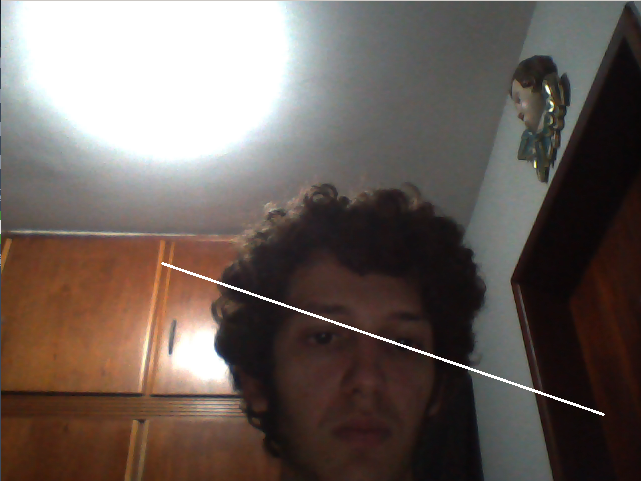
\includegraphics[width=.28\textwidth]{Figs/execution_DP2.png}&
    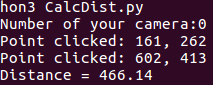
\includegraphics[width=.28\textwidth]{Figs/terminal_DP2.png}\\
    (I)&(II)\\\
    \end{tabular}
    \caption{Resultado do cálculo de distâncias:  (I) Transmissão do vídeo com a reta entre os dois pontos; (II) Saída do terminal}
    \label{fig:Req1}
\end{figure}

Observa-se que o primeiro requesito de se calcular a distância em píxels entre dois pontos por meio do comando do mouse do usuário é cumprido, mostrando a distância euclidiana com precisão em milésimos. 

\subsection{Calibração da Câmera}
\begin{figure}[H]
    \centering
    \begin{tabular}{ccc}
    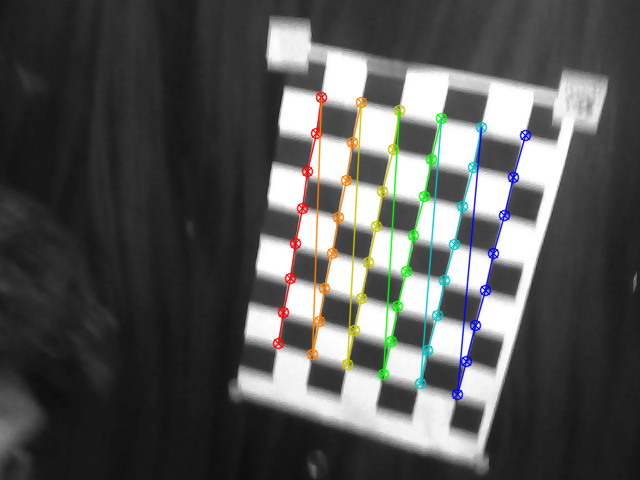
\includegraphics[width=.15\textwidth]{Figs/1_chess.png}&
    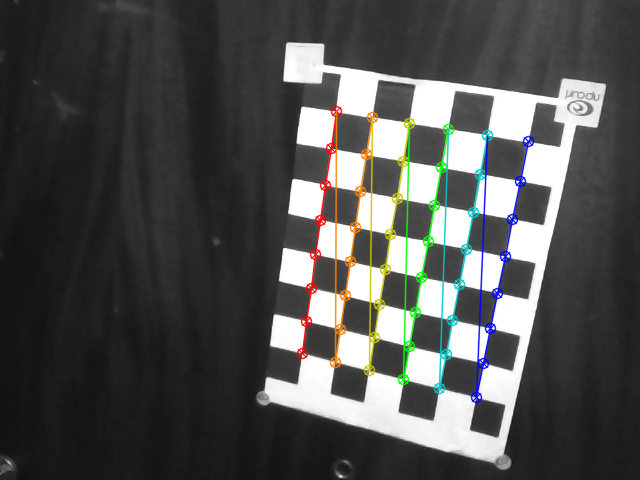
\includegraphics[width=.15\textwidth]{Figs/2_chess.png}&
    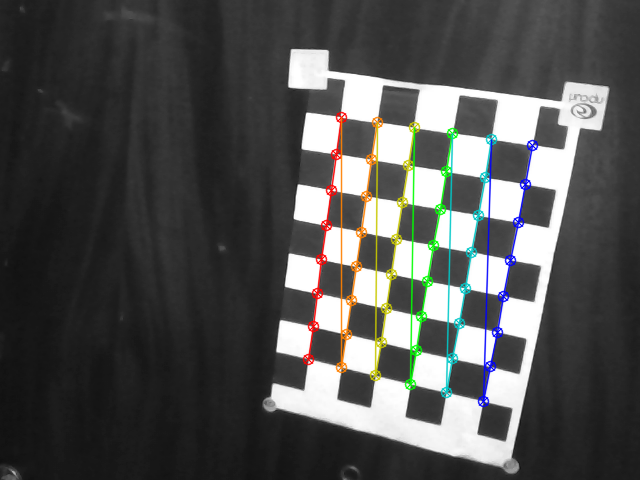
\includegraphics[width=.15\textwidth]{Figs/3_chess.png}&
    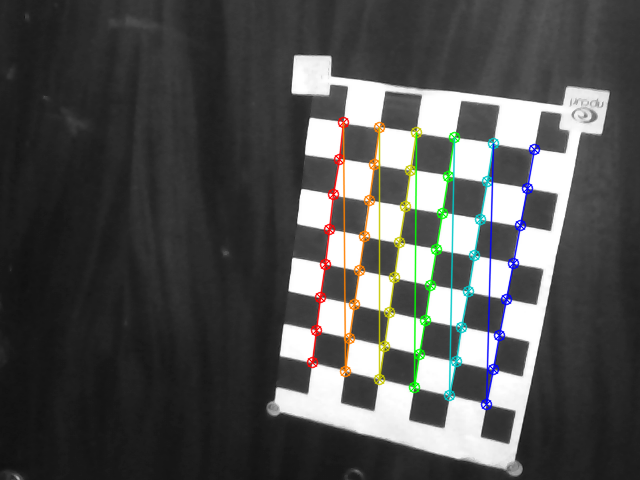
\includegraphics[width=.15\textwidth]{Figs/4_chess.png}&
    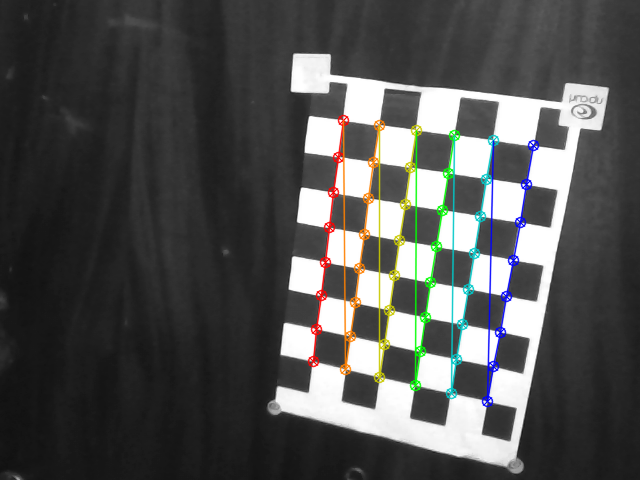
\includegraphics[width=.15\textwidth]{Figs/5_chess.png}
    \end{tabular}
    \caption{Último conjunto de imagens usado para cálculo dos intrísecos}
    \label{fig:calib}
\end{figure}
%Deste padrão, obteve-se as seguintes matrizes de matriz de calibração e matriz de distorção  , respectivamente.\\

Com os dados das outras calibrações, a média e desvio padrão obtidos dos intrínsecos foi, respectivamente:
\[
\begin{bmatrix}
    5.09x10^{2} & 0 & 4.22x10^{2} \\
    0 & 4.73x10^{2} & 1.89x10^{2}\\ 0 & 0  & 1 \\
\end{bmatrix}
\begin{bmatrix}
    6,81 & 0 & 9,25\\
    0 & 10,14 & 3,22\\ 0 & 0  & 0 \\
\end{bmatrix}
\]
E estes foram os dados de média e desvio dos coeficientes de distorção, respectivamente:
\[
\begin{bmatrix}
    2.229x10^{-1} & -3.811x10^{-1} & -2.663x10^{-2} &
    2.95x10^{-2} & 3.02x10^{-1}\\
\end{bmatrix}
\]
\[
\begin{bmatrix}
    7.95x10^{-3} &  4.82x10^{-2} & 9.06x10^{-4} &
    2.40x10^{-3} & 6.50x10^{-2}\\
\end{bmatrix}\]
Para a matriz de extrínsecos, o resultado de média e desvio padrão obtido pode ser visualizado logo abaixo:
\[\begin{bmatrix}
    9,67x10^{-1} & 1,09x10^{-1} & 2,30x10^{-1} & -2.11x10^{2} \\
    -1.82x10^{-1} & 9.26x10^{-1} & 3.29x10^{-1} & 
    -2.088x10^{1}\\ -1.77x10^{-1} & -3.611x10^{-1} & 9.15x10^{-1} & 3.837x10^{2}\\
\end{bmatrix}\]
\[\begin{bmatrix}
    4.45x10^{-4} & 4.83x10^{-3} & 1.67x10^{-3} & 6.06 \\
     3.09x10^{-3} & 1.788x10^{-3} & 6.57x10^{-3} & 
    2.44\\ 1.819x10^{-3} & 6.018x10^{-3} & 2.65x10^{-3} & 6.78\\
\end{bmatrix}\]

Para a implementação da função responsável por desfazer a distorção do padrão de calibração, realizou-se os testes com dois métodos diferentes: utilizando-se a função do OpenCV \href{https://docs.opencv.org/2.4/modules/calib3d/doc/camera_calibration_and_3d_reconstruction.html#getoptimalnewcameramatrix}{getOptimalNewCameraMatrix} e a solução sugerida por Yohai Devir\cite{Devir01}. Trabalhando-se com a função do OpenCV, observa-se a necessidade de que as imagens usadas para a calibração tenham uma diferença bem grande posição angular, observando-se para entradas bem próximas e com pouca distorção apresentada um erro de indeterminação matemática, onde o roi se torna zero. A implementação da função feita por Devir visa tratar os erros de indeterminação encontradas na função do OpenCV por meio de uma implementação utilizando-se do método de Newton-Raphson de estimação de raízes, no qual se mostro bem mais preciso e eliminou os problemas antes presentes.\\
Para o cálculo da distancia, baseou-se na equação geral a seguir:
\begin{equation}
\left[ \begin{array}{l}{u} \\ {v} \\ {1}\end{array}\right]=\left[ \begin{array}{lll}{f_{x}} & {0} & {c x} \\ {0} & {f_{y}} & {c y} \\ {0} & {0} & {1}\end{array}\right][\mathbf{R} | \mathbf{t}] \left[ \begin{array}{c}{X} \\ {Y} \\ {Z} \\ {1}\end{array}\right]
\end{equation}
Onde o vetor X,Y,Z,1, representa a estimativa de posição do objeto, como esse vetor é uma incógnita, calculou-se o vetor, a partir dos parâmetros da câmera, assim, foi necessário calcular a matriz inversa dos parâmetros intrínsecos, gerar a matriz [\mathbf{R} | \mathbf{t}] a partir dos vetores de rotação e de translação, e após isso foi calculada a matriz pseudo inversa desta matriz. Multiplicou-se pela posição do pixel e assim, para determinados dois pixels, foi calculada a distancia pela equação da distancia euclidiana.
\subsection{Régua Visual}
Os resultados mostrados abaixo são referentes à medição de um lápis com comprimeto de 142 mm:
\begin{table}[H]
\centering
\begin{tabular}{|l|l|l|l|}
\hline
Posição do padrão de calibração           & dmin   & dmed  & dmax  \\ \hline
|t|, medida pela trena                    & 48     & 60   & 160   \\ \hline
|t|, calculada pela calibração extrínseca & 47,56  & 58,6 & 150,4 \\ \hline
lraw,centre                               & 160,29 & 124   & 105   \\ \hline
lraw,perifery                             & 186,30 & 136,4 & 100,6 \\ \hline
lundistorted,centre                       & 172,53 & 133   & 115,5 \\ \hline
lundistorted,perifery                     & 194,68 & 146,4 & 110,3 \\ \hline
\end{tabular}
\end{table}
As imagens \ref{fig:Medidas} mostram duas das medidas realizadas:
\begin{figure}[H]
    \centering
    \begin{tabular}{ccc}
    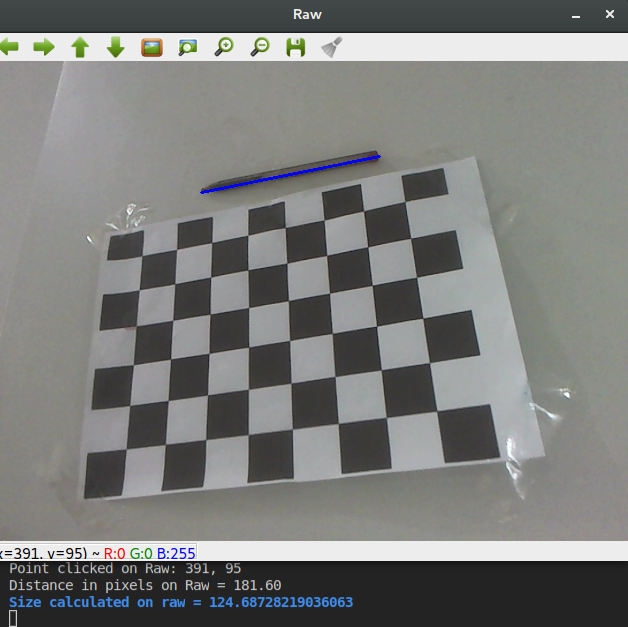
\includegraphics[width=.28\textwidth]{Figs/Dado2.png}&
    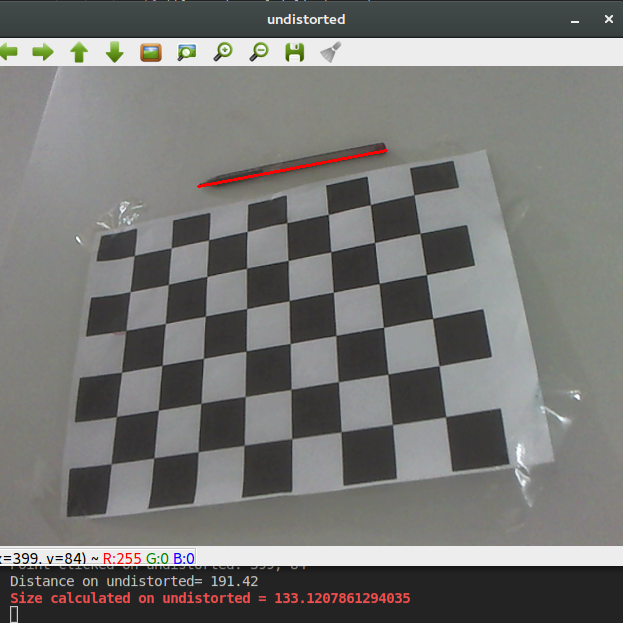
\includegraphics[width=.28\textwidth]{Figs/Dado1.png}\\
    (I)&(II)\\\
    \end{tabular}
    \caption{Medidas obtidas a uma distância de 600 mm:  (I) Transmissão Raw (Com Distorções); (II) Transmissão Undistorted (Sem Distorções)}
    \label{fig:Medidas}
\end{figure}
Percebe-se pelos dados da tabela que quando a medição é feita distante do padrão do xadrez, a medida realizada acaba sendo bastante comprometido. Deve-se isso muito ao efeito de distorção de bordas, onde se tem distorção das lente\cite{Hull01}, algo que deve-se levar em conta quando se mexe com câmeras reais. Outro aspecto notado é de que para regiões muito próximas, o efeito de distorção de bordas apresenta-se em um raio bem menor, comprometendo a medida realizada. Quando a medida realizada é distante, devido ao fato de que os padrões do tabuleiro de xadrez se tornam muito pequenos, causando confusão entre as arestas a serem detectadas, não possibilitando a perfeita captura da medida desejada.\\


\section{Conclusão}

Por meio dos resultados obtidos, pode-se dizer que . No cálculo dos intrínsecos, percebe-se que o seu cálculo torna-se bastante comprometido quando toma-se imagens do padrão do tabuleiro de xadrez muito distante, à ponto de que ele confunda a posição entre as diferentes intersecções.\\
Há muitos fatores que interferem no processo de calibração da câmera, alguns são contornáveis como garantir angulação e diferentes posições do objeto de calibração e outros não são como as imperfeições físicas do objeto e da câmera, ruídos, interferências eletromagnéticas e etc. Foi obtido um resultado condizente, a régua implementada não pode ser usada como instrumento de medição exato, porém os resultados foram em ordens de grandeza aceitáveis e próximas das reais. \\
Foram  implementadas várias técnicas estudadas em sala de aula e o trabalho permitiu a validação das mesmas, além de grande conhecimento na areá de câmeras e calibração.

%-------------------------------------------------------------------------
\newpage
\bibliography{refs}
\end{document}
